%******************************************************************************
% KOMA-Script article scrartcl
%******************************************************************************
\documentclass[11pt, b5paper]{article} 

% Add here all the packages that will be used in the document
%******************************************************************************
% Packages 
%******************************************************************************
% For hyperlinks 
\usepackage{url}

% Add no chapters to the article 
\usepackage[nochapters]{classicthesis}

% Setup the page geometry
\usepackage{geometry}
\geometry{a4paper, total={210mm, 297mm}, 
left=20mm, right=20mm, top=20mm, bottom=20mm}

% Use tikz to add watermarks to the document
\usepackage{blindtext,tikz}
\usetikzlibrary{calc}

% Use the classicthesis style for the style of the document
\usepackage[nochapters]{classicthesis} 

% Use the currvita style for the layout of the document
\usepackage[LabelsAligned]{currvita} 

% Required for adding links	and customizing them
\usepackage{hyperref} 

 % Set link colors
\hypersetup{colorlinks, breaklinks, urlcolor=Maroon, linkcolor=Maroon}


% Add a list of new commands 
%******************************************************************************
% Commands 
%******************************************************************************
\newcommand{\latex}{\LaTeX\xspace}
\newcommand{\tex}{\TeX\xspace}

\usepackage{listings}
\usepackage{color}
\usepackage{graphicx}
\usepackage{caption}
\usepackage{subcaption}

\graphicspath{{images/report7/}}

\definecolor{dkgreen}{rgb}{0,0.6,0}
\definecolor{gray}{rgb}{0.5,0.5,0.5}
\definecolor{mauve}{rgb}{0.58,0,0.82}

\lstset{frame=tb,
  language=Java,
  aboveskip=3mm,
  belowskip=3mm,
  showstringspaces=false,
  columns=flexible,
  basicstyle={\small\ttfamily},
  numbers=none,
  numberstyle=\tiny\color{gray},
  keywordstyle=\color{blue},
  commentstyle=\color{dkgreen},
  stringstyle=\color{mauve},
  breaklines=true,
  breakatwhitespace=true,
  tabsize=3
}

%******************************************************************************
% DOCUMENT STARTS HERE 
%******************************************************************************
\begin{document}

% TITLE 
\title{\rmfamily\normalfont\spacedallcaps{
Report \#{7}
}}

% PROJECT NAME -> ADD YOUR PROJECT NAME HERE
\author{{\small Automatic Mandible Segmentation Using VTK}}

% AUTOMATIC DATE -> DON'T CHANGE MANUALLY
\date{\footnotesize{\today}}

% MAKE THE TITLE -> DON'T CHANGE MANUALLY
\maketitle

% DON'T INCLUDE THE ABSTRACT FOR THE MOMENT
% % \begin{abstract}
% \noindent Abstract
% \end{abstract}
 
%******************************************************************************
% TABLE OF CONTENTS (uncomment to show / comment to hide)
%******************************************************************************     
% \tableofcontents


%******************************************************************************
% Report Content
%******************************************************************************
\section{Report Details}
\begin{center}
\begin{tabular}{ l | c }
\hline 
Report ID & 7  \\ % Change the sprint ID here 
\hline 
Report Duration & 1 Week \\ % Change the duration here 
\hline 
Beginning & 6.12.2016 \\ % Change the start data here
\hline 
End & 13.12.2016 \\ % Change the end data here
\hline 
\end{tabular}
\end{center}

%\section{Objectives}
\section{Original Objectives}
\begin{itemize}
\item Enhance GUI.
\item Maxilla segmentation.
\item Teeth Segmentation.
\item X-Ray Effect.
\end{itemize}

\section{Accomplished Objectives}
\subsection{Enhance GUI}
I have worked on the GUI to improve its functionality and user interactivity, as shown in figure \ref{fig:C15} and \ref{fig:C5} the Volume of interest is selected using some slider and also the threshold can be selected using another slider, the change automatically rendered on the display widget in interactive mannar, I have used different cases for testing they are case 15 and case 5. It is easy to segment the mandible and Maxilla of the dataset,The user just have to change the volume of interest and run segmentation algorithm again.

\subsection{Maxilla Segmentation}
Figure \ref{Fig:C5U1}, \ref{Fig:C5U2}, and \ref{fig:C15U} shows the result of maxilla segmentation for different cases.
\begin{figure}
    \centering
    \begin{subfigure}[b]{0.75\textwidth}
        \centering
        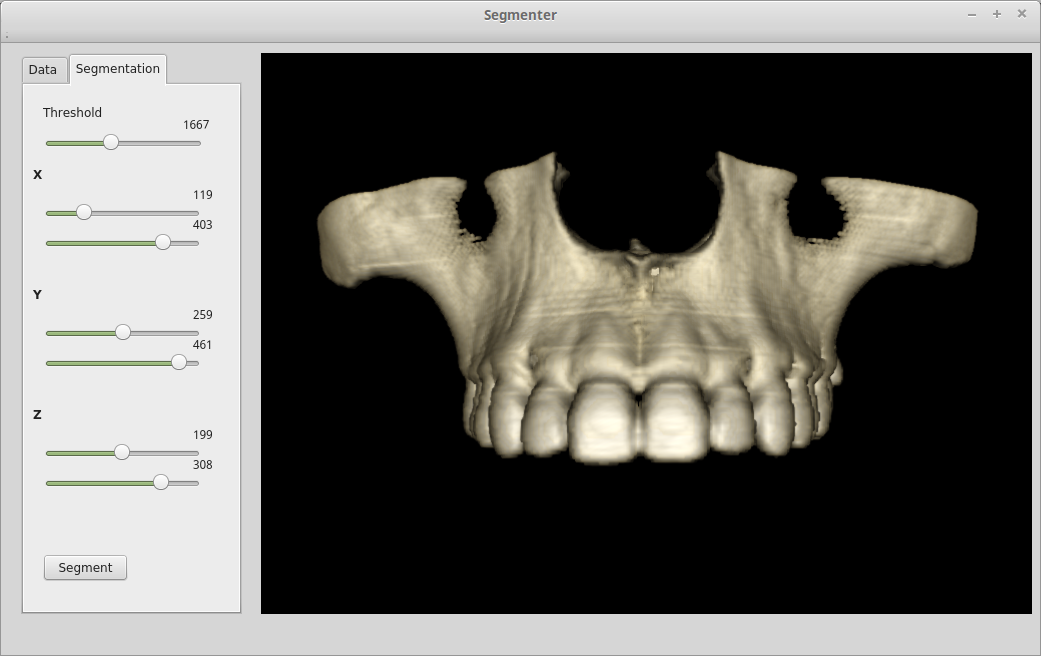
\includegraphics[width=\textwidth]{C15U}
        \caption{Maxilla}
        \label{fig:C15U}
    \end{subfigure}
    \hfill
    \begin{subfigure}[b]{0.75\textwidth}
        \centering
        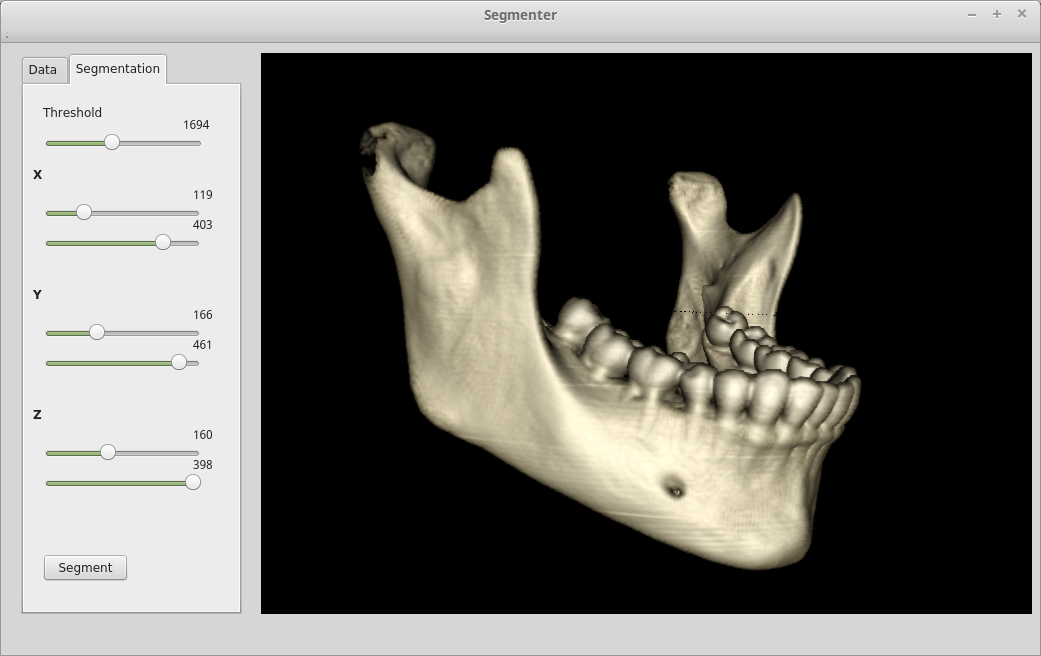
\includegraphics[width=\textwidth]{C15L}
        \caption{Mandible}
    \end{subfigure}
    \caption{Segmentation of Mandible and Maxilla of Case 15}
    \label{fig:C15}
\end{figure}

\begin{figure}
    \centering
    \begin{subfigure}[b]{0.75\textwidth}
        \centering
        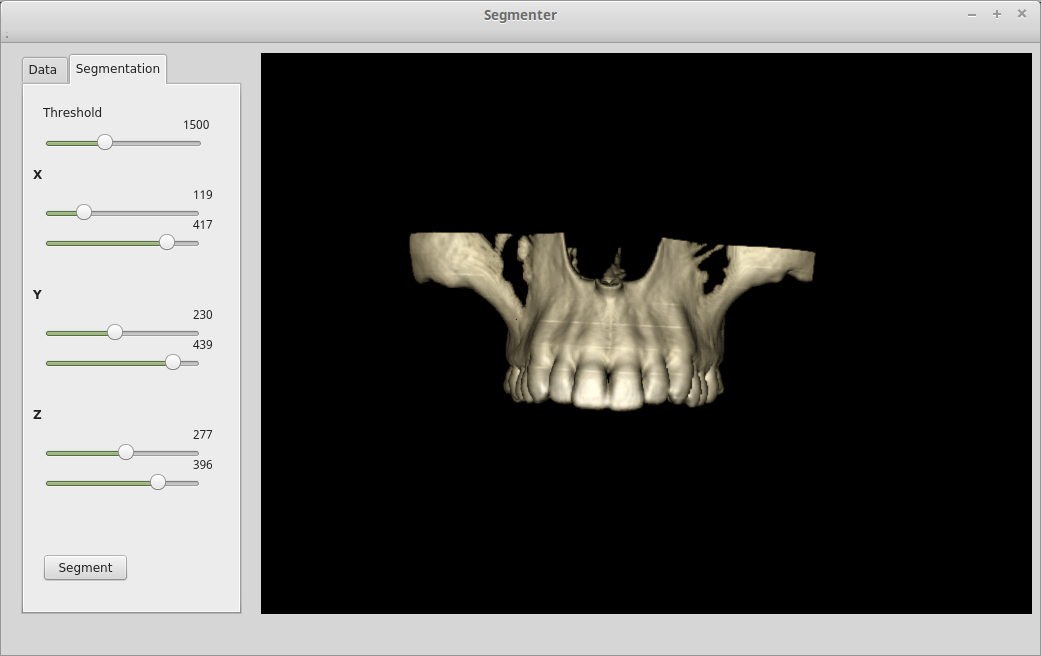
\includegraphics[width=\textwidth]{C5U1}
        \caption{Maxilla}
        \label{Fig:C5U1}
    \end{subfigure}
    \hfill
    \begin{subfigure}[b]{0.75\textwidth}
        \centering
        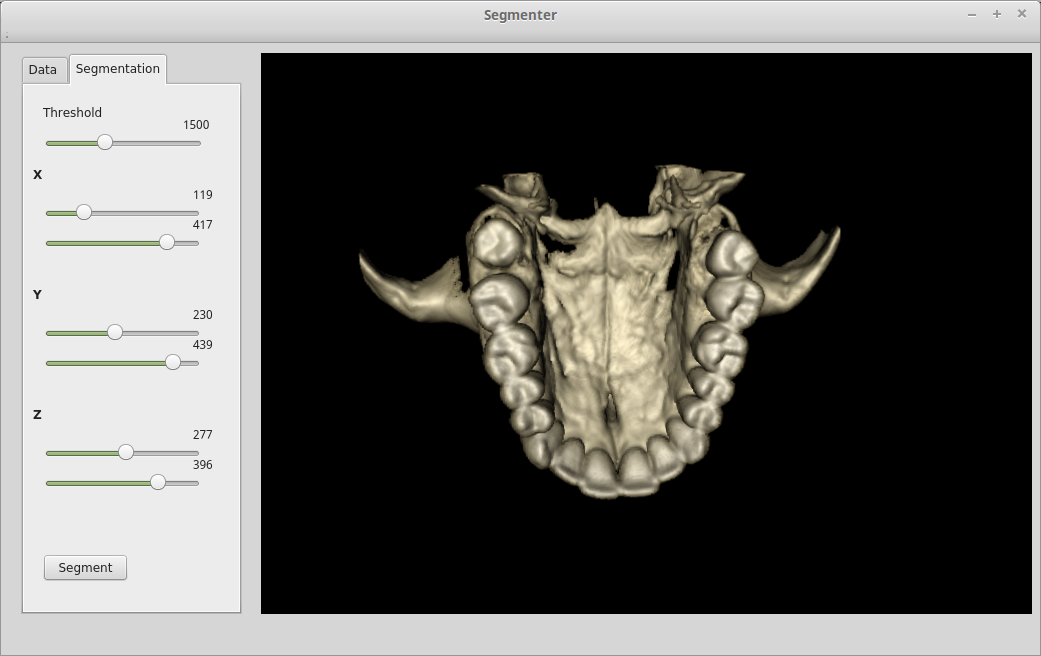
\includegraphics[width=\textwidth]{C5U2}
        \caption{Maxilla}
         \label{Fig:C5U2}
    \end{subfigure}
    \hfill
    \begin{subfigure}[b]{0.75\textwidth}
        \centering
        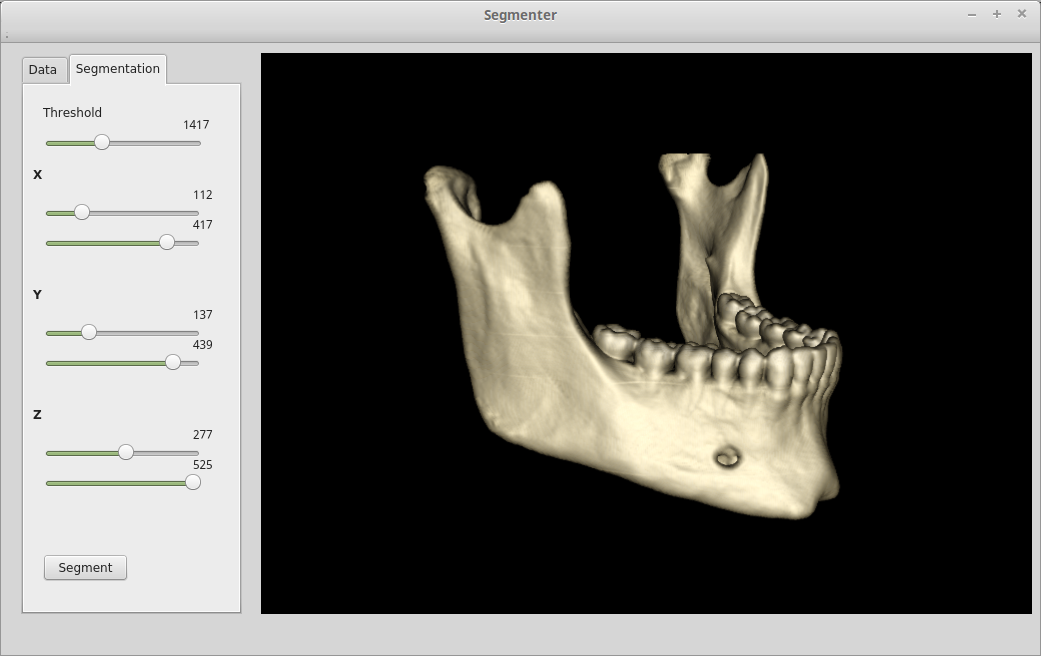
\includegraphics[width=\textwidth]{C5L}
        \caption{Mandible}
    \end{subfigure}
    \caption{Segmentation of Mandible and Maxilla of Case 5}
    \label{fig:C5}
\end{figure}



\section{Missed Objectives}
\begin{itemize}
\item Teeth Segmentation.
\item X-Ray Effect.
\end{itemize}

\section{Next Step}
\begin{itemize}
\item Do missed objectives.
\end{itemize}
%******************************************************************************
% DOCUMENT ENDS HERE 
%******************************************************************************
\end{document}